% Numerical Computing II
% Homework 22
% Initial Value Problems for ODE
% May 2, 2010
% 22.2, 22.3, 22.5, 22.6, 22.8

\documentclass[11pt]{article}
\usepackage{listings}
\usepackage[fleqn]{amsmath}
\usepackage{graphicx}
\usepackage{amsthm}
\begin{document}         
% Start your text
\newcommand{\makehomework}[2]%
{\begin{center}%
	\Huge #1\\%
	\Large #2\\%
	Marty Fuhry\\%
	\today%
\end{center}}
\makehomework{Numerical Computing II}{Homework 22: Initial Value Problems for Ordinary Differential Equations}

\lstset{language=Matlab,numbers=left,frame=single,breaklines=true,morecomment=[l]{//}}
\section*{Exercise 22.2}
To show that the Backwards Euler's Method is $O(h)$, we begin by showing the following:
\begin{flalign*}
    u_n &= (\frac{1}{1-\lambda h})^n u_0\\
        &= (1 + \lambda h + O(h^2))^n u_0\\
    e^{\lambda nh + n O(h^2)}u_0 &= (1 + \lambda h + O(h^2))^nu_0.
\end{flalign*}
So we have equality with $O(h^2)$ between $u_n$ and $e^{n \lambda h + n O(h^2)}$.
Use this equality to solve the global error. Note that $t_n - t_0 = nh$.
\begin{flalign*}
    u_n - u(t_n) &= u_n - u_0e^{\lambda(t_n - t_0)}\\
                 &= u_n - u_0e^{\lambda nh}\\
                 &= u_0 e^{\lambda nh + n O(h^2)} - u_0 e^{\lambda nh}.
\end{flalign*}
We know that $nh = t_n - t_0$ is a constant, so $n O(h^2) = O(nh^2) = (t_n - t_0) O(h) = O(h)$. Then,
\begin{align*}
    e^{n O(h^2)} = e^{O(h)} = 1 + O(h).
\end{align*}
Substituting this in for our global error yields:
\begin{flalign*}
    u_n - u(t_n) &= u_0 e^{\lambda nh} e^{n O(h^2)} - u_0 e^{\lambda nh}\\
                 &= u_0 e^{\lambda nh} e^{O(h)}     - u_0 e^{\lambda nh}\\
                 &= u_0 (1 + O(h)) e^{\lambda nh} - u_0 e^{\lambda nh}\\
                 &= u_0 e ^{\lambda nh} + u_0 O(h) - u_0 e^{\lambda nh}\\
                 &= u_0 O(h)\\
                 &= O(h)
\end{flalign*}
\qedsymbol

\section*{Exercise 22.3}
We need to explicitly solve for $u_1$ in the trapezoidal method $u_1 = 1/2(u_0 + hf(t_0,u_0) + u_1 + hf(t_1,u_1))$.
Multiplying this out and solving $u_1$ gives us:
\begin{flalign*}
    u_1 &= u_0 + \frac{h}{2} (f(t_0,u_0) + f(t_1,u_1))\\
        &= u_0 + \frac{h}{2} (\lambda u_0 + \lambda u_1)\\
        &= u_0 + \frac{h\lambda}{2} u_0 + \frac{h\lambda}{2} u_1\\
    u_1 - \frac{h\lambda}{2} u_1 &= u_0 + \frac{h\lambda}{2}u_0\\
    u_1 ( 1 - \frac{h\lambda}{2}) &= u_0(1 + \frac{h\lambda}{2})\\
    u_1 &= u_0\frac{1 + \frac{h\lambda}{2}}{1 - \frac{h\lambda}{2}}.
\end{flalign*}
Now, we need to manipulate $u_1$ by solving it as a geometric series:
\begin{flalign*}
    u_1 &= u_0(1 + \frac{h\lambda}{2})(\frac{1}{1 - h\lambda})\\
        &= u_0(1 + \frac{h\lambda}{2})(1 + \frac{h\lambda}{2} + (\frac{h\lambda}{2})^2 + (\frac{h\lambda}{2})^3 + O(h^4))\\
        &= u_0(1 + h\lambda + \frac{(h\lambda)^2}{2} + \frac{2(h\lambda)^3}{8} + \frac{(h\lambda)^3}{8} + O(h^4))\\
        &= u_0(1 + h\lambda + \frac{(h\lambda)^2}{2} + \frac{3(h\lambda)^3}{8} + O(h^4)).
\end{flalign*}
Now, using the exponential expansion:
\begin{align*}
    u_0e^{h\lambda} = u_0(1 + h\lambda + \frac{(h\lambda)^2}{2} + \frac{(h \lambda)^3}{6} + O(h^4))
\end{align*}
we can finally solve the local error:
\begin{flalign*}
    u_1 - u(t_1) =& u_0(1 + h\lambda + \frac{(h\lambda)^2}{2} + \frac{3(h\lambda)^3}{8} + O(h^4)) -\\
                  & u_0(1 + h\lambda + \frac{(h\lambda)^2}{2} + \frac{(h \lambda)^3}{6} + O(h^4))\\
                 =& O(h^3).
\end{flalign*}
\qedsymbol
\section*{Exercise 22.5}
\begin{align*}
    u_{j+1} = u_j + h(\alpha u_{j+1}' + \beta u_j')
\end{align*}
We use this method with the conditions $u_l' = f(t_l,u_l)$.
We begin with the function $u(t) = 1$, which means that $f(t_l, u_l) = 0 \forall t_i, u_i$.
Choose $t_0 = 0, t_1 = h$ and then $u(t_0) = 0, u(t_1) = 0$.
\begin{flalign*}
    u_0' &= f(t_0, u_0) = 0\\
    u_1' &= f(t_1, u_1) = 0\\
    u_1  &= u_0 + h(\alpha u_1' + \beta u_0')\\
         &= u_0 + h(\alpha 0    + \beta 0   )\\
    u_1  &= u_0 = 0.
\end{flalign*}
Now we try $u(t) = t$, which means that $f(t_l, u_l) = 1 \forall t_i, u_i$.
Choose $t_0 = 0, t_1 = h$ and then $u(t_0) = 0, u(t_1) = h$.
\begin{flalign*}
    u_0' &= f(t_0, u_0) = 1\\
    u_1' &= f(t_1, u_1) = 1\\
    u_1  &= u_0 + h(\alpha f(t_1, u_1) + \beta f(t_0, u_0))\\
         &= u_0 + h(\alpha 1    + \beta 1   )\\
    h    &= h(\alpha + \beta)\\
    1    &= \alpha + \beta
\end{flalign*}
We have our first equation, then. Now we try $u(t) = t^2$, which means that $f(t_l, u_l) = 2t$.
Choose $t_0 = 0, t_1 = h$ and then $u(t_0) = 0, u(t_1) = h^2$.
\begin{flalign*}
    u_0' &= f(t_0, u_0) = 0\\
    u_1' &= f(t_1, u_1) = 2h\\
    u_1  &= u_0 + h(\alpha u_1' +  \beta u_0')\\
    h^2  &= 0   + h(\alpha 2h   + \beta 0)\\
    h^2  &= \alpha 2h^2\\
    \frac{1}{2} &= \alpha = \beta.
\end{flalign*}
Then, try $u(t) = t^3$, which means that $f(t_l, u_l) = 3t^2$.
Choose $t_0 = 0, t_1 = h$ and then $u(t_0) = 0, u(t_1) = h^3$.
\begin{flalign*}
    u_0' &= f(t_0, u_0) = 0\\
    u_1' &= f(t_1, u_1) = 3h^2\\
    u_1  &= u_0 + h(\alpha u_1' +  \beta u_0')\\
    h^3  &= 0   + h(\alpha 3h^2   + \beta 0)\\
    h^3  &= \alpha 3h^3\\
    \frac{1}{3} &= \alpha \implies \beta = \frac{2}{3}. 
\end{flalign*}
But this doesn't agree with our other equations. 
$\alpha = \beta = 1/2$ works for all polynomials up to and including $t^2$.
When we reach the polynomial $t^3$, we need $\alpha = 1/3$, which conflicts for polynomials of lower degree.
\section*{Exercise 22.6}

Apply each method to:
\begin{align*}
    u'(t) = -25u(t)\\
    t\geq t_0\\
    u(t_0)=u_0.
\end{align*}
\subsubsection*{Trapezoidal Method}
The trapezoidal method is given by:
\begin{align*}
    u_{j+1} = u_j + \frac{h}{2}(f(t_j, u_j) + f(t_{j+1}, u_{j+1})).
\end{align*}
We apply this rule for the function $f(t,u) = \lambda u$ and observe:
\begin{flalign*}
    u_{j+1} &= u_j + \frac{h}{2}(f(t_j, u_j) + f(t_{j+1}, u_{j+1}))\\
            &= u_j + \frac{h}{2}(\lambda u_j + \lambda u_{j+1})\\
            &= u_j + \frac{h}{2}\lambda u_j  + \frac{h}{2}\lambda u_{j+1})\\
    u_{j+1} -\frac{h}{2} \lambda u_{j+1} &= u_j + \frac{h}{2}\lambda u_j\\ 
    u_{j+1} (1 - \frac{h}{2} \lambda) &=    u_j + \frac{h}{2}\lambda u_j\\ 
    u_{j+1} &=    u_j \frac{1 + \frac{h}{2}\lambda}{1 - \frac{h}{2} \lambda} \\ 
    u_{j+1} &=    u_0 (\frac{1 + \frac{h}{2}\lambda}{1 - \frac{h}{2} \lambda})^j.
\end{flalign*}
This converges if and only if
\begin{equation}
    \label{eqn:converge}
    \frac{1 + \frac{h}{2}\lambda}{1 - \frac{h}{2}\lambda} < 1.
\end{equation}
Since $h > 0$ and $\lambda < 0$, (\ref{eqn:converge}) is equivalent to
\begin{align*}
    1 + \frac{h}{2} \lambda < 1 - \frac{h}{2} \lambda\\
    h \lambda < 0\\
    -25 h < 0.
\end{align*}
In this case, it works for all positive $h$.

\subsubsection*{Heun's Method}
Heun's method is given by:
\begin{align*}
    u_{j+1} = u_j + \frac{h}{2}(f(t_j,u_j) + f(t_{j+1}, \hat{u_{j+1}})).
\end{align*}
Note that $\hat{u_{j+1}}$ is taken from Euler's method
\begin{align*}
    \hat{u_{j+1}} = u_j + hf(t_j,u_j). 
\end{align*}
Rewriting Heun's method, we get:
\begin{align*}
    u_{j+1} = u_j + \frac{h}{2}(f(t_j,u_j) + f(t_{j+1}, u_j + hf(t_j,u_j))).
\end{align*}
We apply this rule for our function given by $f(t,u) = \lambda u$ and observe:
\begin{flalign*}
    u_{j+1} &= u_j + \frac{h}{2}(f(t_j,u_j) + f(t_{j+1}, u_j + hf(t_j,u_j)))\\
            &= u_j + \frac{h}{2}(f(t_j,u_j) + f(t_{j+1}, u_j + h \lambda u_j))\\
            &= u_j + \frac{h}{2}(\lambda u_j + \lambda (u_j + h \lambda u_j))\\
            &= u_j + \frac{h}{2}(2 \lambda u_j + h \lambda^2 u_j))\\
            &= u_j + h \lambda u_j + \frac{h^2}{2} \lambda^2 u_j))\\
            &= u_j(1  + h \lambda + \frac{h^2}{2} \lambda^2)\\
            &= u_0(1  + h \lambda + \frac{h^2}{2} \lambda^2)^j.
\end{flalign*}
This converges if and only if
\begin{flalign*}
     1  + h \lambda + \frac{h^2}{2} \lambda^2 <& 1\\
     2h \lambda + h^2 \lambda^2 <& 0\\
     h\lambda(2 + h\lambda) <& 0.
\end{flalign*}
Since $h \lambda < 0$, we need $2 + h \lambda > 0$ to satisfy the inequality. Then,
\begin{flalign*}
     2 + h\lambda >& 0\\
     h \lambda > -2\\
     h < \frac{2}{25}.
\end{flalign*}
We get this from $\lambda = -25$. So, when $h < \frac{2}{25}$, Heun's method converges in this case.

\subsubsection*{Example 22.7: Explicit Multistep Method}
The Explicit Multistep Method from Example 22.7 is given by
\begin{align*}
    u_{j+1} = u_j + h(\alpha u_j' + \beta u_{j-1}').
\end{align*}
Use the fact that $u_l' = f(t_l, u_l) = \lambda u_l$, and apply this rule for $f(t,u) = \lambda u$.
\begin{flalign*}
    u_{j+1} &= u_j + h(\alpha u_j' + \beta u_{j-1}')\\
            &= u_j + h(\alpha \lambda u_j + \beta \lambda u_{j-1})\\
            &= u_j + h\alpha \lambda u_j + h\beta \lambda u_{j-1}.
\end{flalign*}
We can't solve explicitly for this function since it is implicit, but we can use our knowledge of the values
of $u_j$ and $u_{j-1}$ to show that since $\lambda = -25$, we have a decreasing function. 
Therefore, $u_j < u_{j-1}$. Now, we have an upper bound on our $u_{j+1}$ value.
\begin{flalign*}
    u_{j+1} &= u_j + h\alpha \lambda u_j + h\beta \lambda u_{j-1}\\
            &<  u_{j-1} (1 + h \alpha \lambda + h \beta \lambda).
\end{flalign*}
This inequality is equal to
\begin{align*}
    u_0 ( 1 + h\alpha \lambda + h \beta \lambda)^{j-1}
\end{align*}
which converges if and only if
\begin{flalign*}
    1 + h\alpha \lambda + h \beta \lambda) &< 1\\
    h\alpha \lambda + h \beta \lambda) &< 0\\
    h\lambda(\alpha + \beta) &< 0\\
    h(\alpha + \beta) &> 0.
\end{flalign*}
Notice the inequality was flipped since $\lambda = - 25$. So this converges if $h$ is positive and the 
sum of the coefficients $\alpha + \beta$ is positive.

\subsubsection*{Conclussions}
The only method which required $h$ to be small was Heun's Method. Both the Trapezoidal Method and 
the Explicit Multistep Method from Example 22.7 converged for all positive values of $h$ (so long 
as the sum of the coefficients $\alpha + \beta$ was positive for the Explicit Multistep Method).
Therefore, both the Trapezoidal Method and the Explicit Multistep Method allowed the largest step length
by not setting any bounds on the size of $h$.

\section*{Exercise 22.8}
% Import Program 
%\lstinputlisting{problem_17_1.m}

% Import Graph
%\begin{center}
%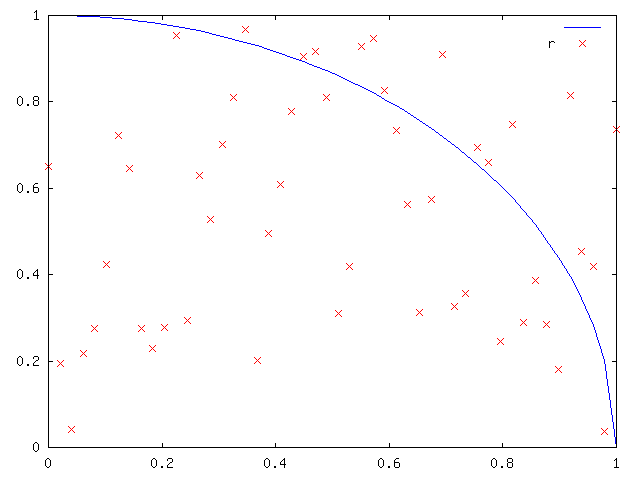
\includegraphics[scale=0.5]{problem_17_1_graph.png}
%\end{center}

% Stop your text
\end{document}
